
\documentclass[12pt]{article}
%\usepackage{geometry} % see geometry.pdf on how to lay out the page. There's lots.
%\geometry{a4paper} % or letter or a5paper or ... etc
% \geometry{landscape} % rotated page geometry
\usepackage{amsmath, aas_macros, graphicx}

% See the ``Article customise'' template for come common customisations

\title{Alternative way to drive slow mode in AstroGK: Laplace-Fourier analysis}
\author{Yuguang Tong}
%\date{} % delete this line to display the current date

%%% BEGIN DOCUMENT
\begin{document}

\maketitle

\section{Gyrokinetic and Maxwell's equations}
Fourier transformed gyrokinetic equation:
%
\begin{equation}
\frac{\partial g_{\mathbf{k}s}}{\partial t} + i k_\parallel v_\parallel g_{\mathbf{k}s} + \frac{q_s}{T_s} v_\parallel F_{0s} i k_\parallel\tilde{\phi} = -\frac{q_s}{T_s} F_{0s} \frac{\tilde{A}}{\partial{t}}
\label{eq:gk_eq_1}
\end{equation}
%
where $\tilde{\phi}$ and $\tilde{A}$ are the source terms:
%
\begin{eqnarray}
\tilde{\phi} & = & j_0(k_\perp \rho_{\perp s})\phi_\mathbf{k}
 +  \frac{J_1(k_\perp \rho_{\perp s})}{k_\perp \rho_{\perp s}}\frac{mv_\perp^2}{q_s} 
\frac{\delta B_{\parallel\mathbf{k}}}{B_0} \\
\tilde{A} & =& J_0\left( k_\perp \rho_{\perp s}\right) \frac{v_\parallel A_{\parallel\mathbf{k}}}{c}
\end{eqnarray}
%
where $\rho_{\perp s} = v_{\perp}/\Omega_{cs}$. 

%%
The Poisson equation:
\begin{equation}
\begin{split}
\sum_s \frac{q_s^2 n_s}{T_s} (1 - \Gamma_{0s}(\alpha_s)) & \phi_\mathbf{k} - \sum_s q_s n_s \Gamma_{1s} (\alpha_s) \frac{\delta B_{\parallel \mathbf{k}}}{B_0} \\
&\quad  = \sum_s q_s \int d^3 \mathbf{v} J_0(k_\perp \rho_{\perp s}) g_{\mathbf{k}s}
\end{split}
\label{eq:poisson_eq_1}
\end{equation}

%%
The parallel component of Ampere's law
\begin{equation}
\frac{ck_\perp^2}{4\pi} A_{\parallel\mathbf{k}} = \sum_s q_s \int d^3\mathbf{v} v_\parallel J_0(k_\perp \rho_{\perp s}) g_{\mathbf{k}s}
\label{eq:par_ampere_1}
\end{equation}
where $\alpha_s = k_\perp^2 \rho_s^2/2$.

%%
The perpendicular component of Ampere's law
\begin{equation}
\begin{split}
\sum_s q_s n_s \Gamma_{1s}(\alpha_s) \phi_\mathbf{k} +  \frac{\delta B_{\parallel \mathbf{k}}}{B_0} \left( \frac{B_0^2}{4\pi} + \sum_s n_sT_s\Gamma_{2s}(\alpha_s)\right) = \\
-\sum_s T_s \int d^3\mathbf{v} \frac{v_\perp^2}{v_{ts}^2}\frac{2J_1(k_\perp \rho_{\perp s})}{k_\perp \rho_{\perp s}} g_{\mathbf{k}s}
\end{split}
\label{eq:perp_ampere_1}
\end{equation}
%%%% section


\section{Driving through phase space density perturbation: I}
( Adapted from Jason TenBarge's note)

Rather than driving $B_\parallel$ to generate slow modes, let us consider driving $\delta_1 U_\parallel$ the bulk parallel flow. This will manifest as a perturbation on the distribution function, $g^{tot}_s = g_s + g_{as}$, where $g_{as}$ denotes antenna driven perturbation. Note that each species must be driven separately to avoid generating a large $J_\parallel$ in Ampere's law, which would drive Alfv{\'e}n waves. An appropriate form for this term is
%
\begin{equation}
g_{as} =u_0(t)Z(z)\Psi(x, y) \frac{v_{\parallel s} e^{-v_s^2/v_{ts}^2} n_s}{N_{u,s} \pi^{3/2} v_{ts}^4} = u_0(t) Z(z) \Phi(x, y) \frac{\hat{v}_{\parallel s} F_{0s}}{N_{u,s}}
\end{equation}
where 
%
\begin{equation}
N_{u,s} = \frac{\hat{v}_{ts}}{\pi^{3/2}} \int d^3 \hat{v}_s J_0\left( \hat{k}_{\perp s} \hat{v}_{\perp s}\right) \hat{v}_{\parallel s} e^{-\hat{v}_s^2}  = \frac{1}{2}\hat{v}_{ts} e^{-\hat{k}_{\perp s}^2 /4}
\end{equation}
and $\hat{v}_{ts} = v_{ts}/v_{t0}$, $\hat{v}_{\parallel s} = v_{\parallel s}/ v_{ts}$, $\hat{k}_{\perp s} = k_\perp \rho_s$.

Now we add this antenna to the gyrokinetic equation and to the Maxwell's equations. To simplify the Fourier-Laplace solution, we assume
%
\begin{equation}
u_0(t) Z(z)\Psi(x, y) = u_0 e^{i (\mathbf{k}_0 \cdot \mathbf{r}-\omega_0 t)}
\end{equation}

Therefore the phase space perturbation takes the form
\begin{equation}
g_{as} = u_0  e^{i (\mathbf{k}_0 \cdot \mathbf{r}-\omega_0 t)} \frac{2 v_{\parallel s} v_{t0}}{v_{ts}^2} F_{0s} e^{(k_\perp \rho_s)^2/4}
\end{equation}
whose spatial Fourier transform is
%
\begin{equation}
g_{\mathbf{k}as} = u_{\mathbf{k}0} e^{-i\omega_0 t}  \frac{2 v_{\parallel s} v_{t0}}{v_{ts}^2} F_{0s} e^{(k_\perp \rho_s)^2/4}
\label{eq:gkas_1}
\end{equation}
and whose Fourier-Laplace transform is
%
\begin{equation}
\hat{g}_{\mathbf{k}as} = \int_0^\infty g_{\mathbf{k}as} e^{-pt} dt = \frac{u_{\mathbf{k}0}}{p+i\omega_0} \frac{2 v_{\parallel s} v_{t0}}{v_{ts}^2} F_{0s} e^{(k_\perp \rho_s)^2/4}
\label{eq:gkas_1}
\end{equation}



\subsection{Fourier-Laplace solution}
We replace $g_{\mathbf{k}s}$ in Eq. (\ref{eq:gk_eq_1}) by $g_{\mathbf{k}s}^{tot}=g_{\mathbf{k}s} +g_{\mathbf{k}as}  $. Take Laplace transform of Eq. (\ref{eq:gk_eq_1}):
%
\begin{equation}
(p + i k_\parallel v_\parallel) \hat{g}_{\mathbf{k}s}^{tot} - g_{\mathbf{k}s}^{tot} (t=0) + \frac{q_s}{T_s} v_\parallel F_{0s} i k_\parallel \hat{\tilde{\phi}} = -\frac{q_s}{T_s}F_{0s} \left(p \hat{\tilde{A}} - \tilde{A} (t=0)\right)
\end{equation}

Since this is a driven system, we can choose initial condition to simplify the solutions as much as possible,  $\tilde{A} (t=0)=0$ and $g_{\mathbf{k}s}^{tot} (t=0) = 0$. 

Therefore, the perturbed distribution function $\hat{g}_{\mathbf{k}s}$ written in terms of fields takes the form:
\begin{equation}
\hat{g}_{\mathbf{k}s}  = -\hat{g}_{\mathbf{k}as} - \frac{1}{{p+ ik_\parallel v_\parallel}} \left(\frac{q_s}{T_s} v_\parallel F_{0s} i k_\parallel \hat{\tilde{\phi}} + \frac{q_s}{T_s}F_{0s} p \hat{\tilde{A}} \right)
\end{equation}

To solve for fields, we substitute the above expression into the Maxwell's equations, i.e., Eq. (\ref{eq:poisson_eq_1}) - (\ref{eq:perp_ampere_1}). To utilize what we already know to simplify derivation, we notice that if the antenna term $\hat{g}_{\mathbf{k}as}$ is absent, the Maxwell's equations take the familiar form of Eq. (4.85) in AstroGK manual, describing a homogeneous gyrokinetic system without driving. We simply need to add moments of $\hat{g}_{\mathbf{k}as}$ to Eq. (4.85) to obtain field equations in a driven system. 
\subsubsection{Poisson's equation}
The antenna contribution to Eq. (\ref{eq:poisson_eq_1}) would be on the RHS:
%
\begin{equation}
\sum_s q_s \int d^3 v J_0(k_\perp \rho_{\perp s}) \hat{g}_{\mathbf{k}as} 
\end{equation}
However, this term vanishes. To show this, we notice that integrand of $v_\parallel$ integral has integrand $v_\parallel  e^{v_\parallel^2/v_{ts}^2}$ ( see Eq. (\ref{eq:gkas_1})). Since the integrand is an odd function, and the integration limit is $(-\infty, \infty)$, the integral vanishes. Hence the antenna term leaves the Poisson equation unchanged.

\subsubsection{Perpendicular Ampere's law}
The antenna term does not modify Ampere's law for the same reason as above.

\subsubsection{Parallel Ampere's law}
We again consider antenna's contribution to the RHS:
%
\begin{eqnarray}
RHS_{ant} &=& -\sum_s q_s \int d^3 v  v_\parallel J_0(k_\perp \rho_{\perp s}) \hat{g}_{\mathbf{k}as} \nonumber \\
&=& \sum_s q_s \int d^3 v  v_\parallel J_0(k_\perp \rho_{\perp s}) \left[ -\frac{u_{\mathbf{k}0}}{p+i\omega_0} \frac{2 v_{\parallel s} v_{t0}}{v_{ts}^2} F_{0s} e^{(k_\perp \rho_s)^2/4}\right] \nonumber \\
&=&\sum_s -\frac{q_s u_{k0} n_{0s}}{p+i\omega_0} \frac{2v_{t0}}{v_{ts}^2} e^{(k_\perp \rho_s)^2/4} I_\parallel I_\perp
\end{eqnarray}
where
%
\begin{equation}
I_\parallel = \int_{-\infty}^{\infty} dv_\parallel v_\parallel^2 e^{-v_\parallel^2 /v_{ts}^2} = \frac{\sqrt{\pi}}{2} v_{ts}^3
\end{equation}
and
%
\begin{eqnarray}
I_\perp &=& \int_0^{\infty} \frac{2\pi} {\pi^{3/2} v_{ts}^3} v_\perp d v_\perp J_0\left( k_\perp \rho_s \frac{v_\perp}{v_{ts}}\right) e^{-v_\perp^2 / v_{ts}^2} \nonumber \\
&=& \frac{2}{\sqrt{\pi} v_{ts}} \int_0^{\infty} x dx J_0(k_\perp \rho_s x) e^{-x^2} \nonumber \\
&=& \frac{e^{-(k_\perp \rho_s)^2/4}}{\sqrt{\pi} v_{ts}}
\label{eq:i_perp_1}
\end{eqnarray}

Therefore
\begin{equation}
RHS_{ant} = \sum_s - \frac{q_s u_{k0} n_{0s} v_{t0}}{p+ i\omega_0}
\end{equation}
Since the plasma is quasi-neutral, the above expression vanishes as well.

\subsubsection{Implication}
The source term $g_{\mathbf{k}as}$ does not enter the Maxwell's equations. Hence in the Fourier-Laplace space, the Maxwell equation takes exactly the same homogeneous form as Eq. (6.104) in AstroGK manual. It is easy to see by evaluating Bromwich integral that all the fields remains zero. 

\subsection{Comparison with AstroGK}
Jason TenBarge implemented the above antenna in AstroGK. Figure \ref{fig:bpar_t_1} shows that energy in $\delta B_\perp$ grows with time and saturates under the antenna driving. The caption gives a detailed description of the plasma parameters. Diagnostic by magnetic variance anisotropy (MVA) that the energy is injected into the slow mode successfully. A decay run (not shown) also shows that Alfv{\'e}n energy are several orders of magnitude lower than slow mode energy. 

It is puzzling that while Fourier-Laplace solution predicts that the fields should vanish, the AstroGK seem to drive slow mode perfectly. As an attempt to reconcile this, we add the same antenna term  to the gyrokinetic equation directly, without letting it enter through the distribution function $g$. 

\begin{figure}
\centering
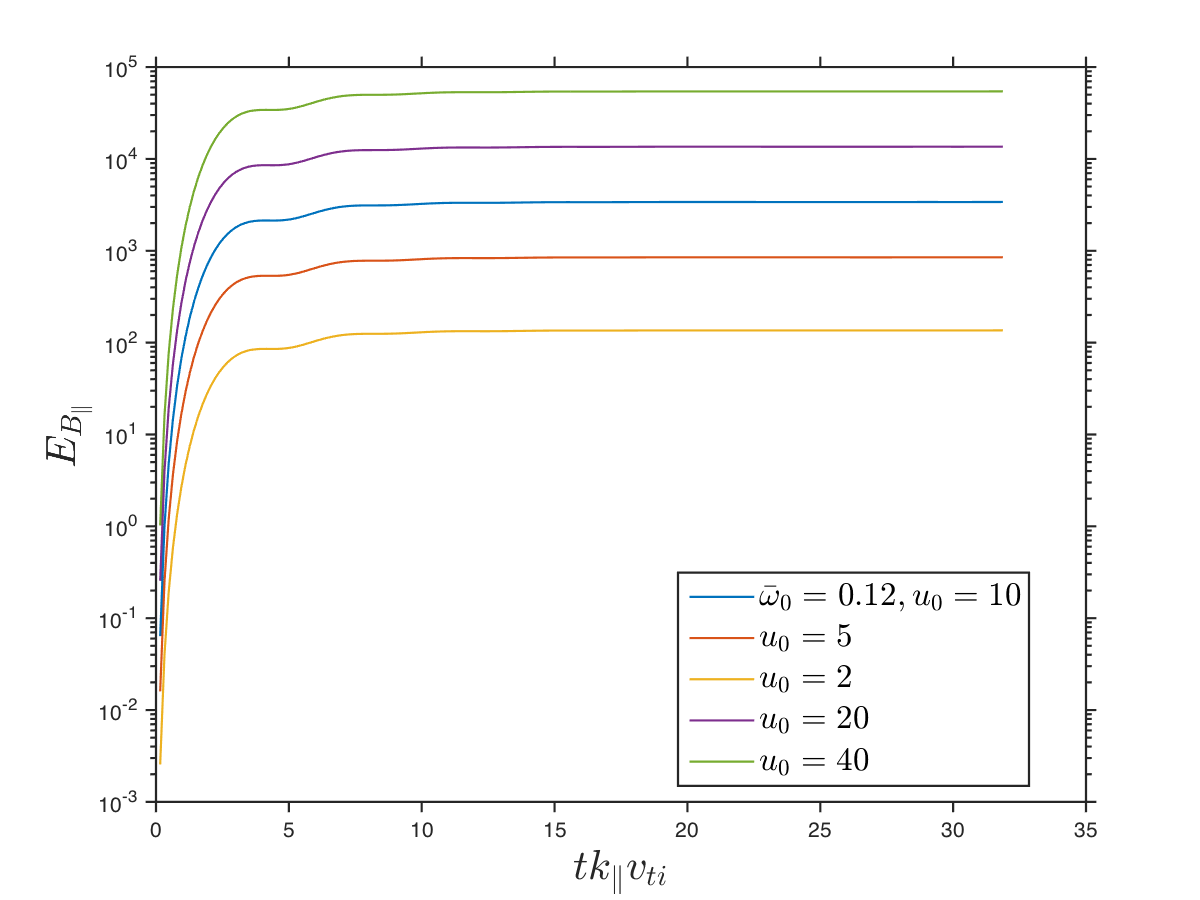
\includegraphics[width=0.8\textwidth]{figure/Ebpar_t_u0_1.png}
\caption{AstroGK linear run with an antenna term in Eq. \ref{eq:gkas_1}. The plasma has $\beta_p = 0.01, T_e = T_p$  which we drive with perturbation $\overline{\omega}_0 = \omega/ k_\parallel v_A = 0.12$ and various amplitudes. The energy of the excited modes are dominated in parallel magnetic field fluctuations, and are proportional to the driving amplitudes. The magnetic variance anisotropy $MVA = \langle |\delta B_\perp |^2\rangle / \langle |\delta B_\parallel|^2 \rangle = 0.019$ in the simulations. In comparison, hot plasma Vlasov-Maxwell's solution gives $MVA=0.024$ for slow mode. }
\label{fig:bpar_t_1}
\end{figure}

\section{Driving through phase space density perturbation: II}
In this section, we try to add antenna term in a different place in the gyrokinetic equation:
%
\begin{equation}
\frac{\partial g_{\mathbf{k}s}}{\partial t} + i k_\parallel v_\parallel g_{\mathbf{k}s} + \frac{q_s}{T_s} v_\parallel F_{0s} i k_\parallel\tilde{\phi} = -\frac{q_s}{T_s} F_{0s} \frac{\tilde{A}}{\partial{t}} + g_{\mathbf{k}, ant, s}
\end{equation}
where $g_{\mathbf{k}, ant, s} = u_{\mathbf{k}0} e^{-i\omega_0 t}  \frac{2 v_{\parallel s} v_{t0}}{v_{ts}^2} F_{0s} e^{(k_\perp \rho_s)^2/4}$ is the same as the antenna term in Eq. (\ref{eq:gkas_1}). We point out that the constant term in the two equations are different since the antenna term is no longer inside time derivative in the above equation. 

Applying Laplace transform to the gyrokinetic equation yields:
%
\begin{equation}
(p + i k_\parallel v_\parallel) \hat{g}_{\mathbf{k}s} - g_{\mathbf{k}s}(t=0) + \frac{q_s}{T_s} v_\parallel F_{0s} i k_\parallel \hat{\tilde{\phi}} = -\frac{q_s}{T_s}F_{0s} \left(p \hat{\tilde{A}} - \tilde{A} (t=0)\right)  + \hat{g}_{\mathbf{k}, ant, s}
\end{equation}
In the driving simulation, the initial fields and distribution perturbation all vanishes, hence we have:
%
\begin{equation}
\hat{g}_{\mathbf{k}s}  = -\frac{1}{p + ik_\parallel v_\parallel} \left(\frac{q_s}{T_s} v_\parallel F_{0s} i k_\parallel \hat{\tilde{\phi}} + \frac{q_s}{T_s}F_{0s} p \hat{\tilde{A}}\right) + \frac{ \hat{g}_{\mathbf{k}, ant, s}}{p + ik_\parallel v_\parallel}
\label{eq:hat_g_ks_1}
\end{equation}
where 
\begin{equation}
\hat{g}_{\mathbf{k}, ant, s} = \int_0^\infty g_{\mathbf{k}as} e^{-pt} dt = \frac{u_{\mathbf{k}0}}{p+i\omega_0} \frac{2 v_{\parallel s} v_{t0}}{v_{ts}^2} F_{0s} e^{(k_\perp \rho_s)^2/4}
\label{eq:gkas_2}
\end{equation}

Next we substitute the Eq. (\ref{eq:hat_g_ks_1}) into the Maxwell's equations to obtain a set of self consistent equations for the fields.
\subsection{Antenna contribution to Maxwell's equations}
In this section, we only consider the modification to the Maxwell's equation by the additional antenna term, and leave the full Maxwell's equations to the next section. 
\subsubsection{Poisson equation}
%
\begin{eqnarray}
\mathrm{RHS}_{ant} &=& \sum_s q_s \int d^3 v J_0(k_\perp \rho_{\perp s}) \frac{1}{p + ik_\parallel v_\parallel} \frac{u_{k0}}{p + i \omega_0} \frac{2 v_\parallel v_{t0}}{v_{ts}^2} F_{0s} e^{(k_\perp \rho_s)^2 / 4} \nonumber \\
&=& \sum_s \frac{u_{k0} q_s}{p + i \omega_0} \frac{v_{t0}}{v_{ts}^2} e^{(k_\perp \rho_s)^2 / 4} I_\parallel I_\perp
\end{eqnarray}
where
%
\begin{eqnarray}
I _\parallel &=& \int d v_\parallel  \frac{2 v_\parallel}{p + i k _\parallel v_\parallel} e^{-v_\parallel^2/v_{ts}^2} \nonumber \\
&=& v_{ts} \int_{-\infty}^{\infty} dt \frac{2t e^{-t^2}}{\frac{p}{v_ts} + ik_\parallel t} \nonumber \\
&=& \frac{2\sqrt{\pi} v_{ts}}{ik_\parallel} \frac{1}{\sqrt{\pi}}\int dt \frac{-te^{-t^2}}{\xi_s - t} \nonumber \\
&=&  \frac{2\sqrt{\pi} v_{ts}}{ik_\parallel} (1 + \xi_s Z_s) = -\frac{\sqrt{\pi} v_{ts}}{ik_\parallel} Z^\prime_s
\label{eq:i_par_1}
\end{eqnarray}
where $Z$ is the plasma dispersion function, $Z^\prime$ its derivative, $\xi_s = \frac{p}{-ik_\parallel v_ts}$ and $Z_s = Z(\xi_s)$.

And 
\begin{eqnarray}
I_\perp &=& \int dv_\perp 2\pi v_\perp J_{0s} e^{-v_\perp^2/v_{ts}^2}\frac{n_{0s}}{\pi^{3/2}v_{ts}^3} \nonumber \\
&=& \frac{n_{0s} e^{-(k_\perp \rho_s)^2/4}}{\sqrt{\pi} v_{ts}}
\label{eq:i_perp_2}
\end{eqnarray}
whose derivation is the same as Eq. (\ref{eq:i_perp_1})

Therefore, 
\begin{equation}
\mathrm{RHS}_{ant} = \sum_s  - \frac{q_s n_{0s} u_{k0}}{p + i \omega_0} \frac{v_{t0}}{ik_\parallel v_{ts}^2} Z^\prime_s
\end{equation}


\subsubsection{Parallel component of Ampere's law}
\begin{eqnarray}
\mathrm{RHS}_{ant} &=& \sum_s q_s \int d^3 v v_\parallel  J_{0s} \hat{g}_{\mathbf{k}, ant, s} \nonumber \\
&=& \sum_s q_s \int d^3 v v_\parallel J_{0s} \frac{u_{k0}}{p + i\omega_0} \frac{2v_\parallel}{p + i k_\parallel v_\parallel} \frac{v_{t0}}{v_{ts}^2} F_{0s} e^{(k_\perp \rho_s)^2/4} \nonumber \\
&=& \sum_s \frac{q_s v_{t0}}{v_{ts}^2} \frac{u_{k0}}{p + i\omega_0} e^{(k_\perp \rho_s)^2/4} I_\parallel I_\perp
\end{eqnarray}
where
\begin{eqnarray}
I_\parallel &=& \int dv_\parallel \frac{2 v_\parallel^2}{p + ik_\parallel v_\parallel} e^{-v_\parallel^2/v_{ts}^2} \nonumber \\
&=& \frac{2\sqrt{\pi}v_{ts}^2}{ik_\parallel} \frac{1}{\sqrt{\pi}}\int dt \frac{-t^2}{\xi-t} e^{-t^2} \nonumber \\
&=& -\frac{\sqrt{\pi}v_{ts}^2}{ik_\parallel} \xi_s Z^\prime_s  
\end{eqnarray}
and $I_\perp$ is exactly the same as in Eq. (\ref{eq:i_perp_2}). Therefore, the antenna term contribute to the parallel Ampere's law through:
\begin{equation}
\mathrm{RHS}_{ant} = \sum_s - \frac{q_s n_{0s} u_{k0}}{ik_\parallel(p + i\omega_0)} \frac{v_{t0}}{v_{ts}} \xi_s Z^\prime_s
\end{equation}

\subsubsection{Perpendicular component of Ampere's law}
\begin{eqnarray}
\mathrm{RHS}_{ant} &=&  -\sum_s T_s \int d^3 v \frac{v_\perp^2}{v_{ts}^2} \frac{2J_{1s}}{k_\perp \rho_{\perp s}} \hat{g}_{\mathbf{k}, ant, s} \nonumber \\
&=& -\sum_s T_s \int d^3 v \frac{v_\perp^2}{v_{ts}^2} \frac{2J_{1s}}{k_\perp \rho_{\perp s}} \frac{1}{p + ik_\parallel v_\parallel} \frac{u_{k0}}{p + i \omega_0} \frac{2 v_\parallel v_{t0}}{v_{ts}^2} F_{0s} e^{(k_\perp \rho_s)^2 / 4} \nonumber \\
&=& - \sum_s \frac{T_s u_{k0} v_{t0}}{(p + i\omega_0) v_{ts}^4} e^{(k_\perp \rho_s)^2/4} I_\parallel I_\perp
\end{eqnarray}
where $I_\parallel$ is exactly the same as Eq. (\ref{eq:i_par_1}) and
\begin{eqnarray}
I_\perp  &=& \int dv_\perp 2\pi v_\perp v_\perp^2 \frac{2J_{1s}}{k_\perp \rho_{\perp s}} \frac{n_{0s}}{\pi^{3/2} v_{ts}^3} e^{-v_\perp^2/v_{ts}^2} \nonumber \\
&=& \int d v_\perp \frac{4\pi n_{0s}}{\pi^{3/2}} \frac{v_\perp^3}{v_{ts}^3} \frac{J_1\left(k_\perp \rho_s \frac{v_\perp}{v_{ts}}\right)}{k_\perp \rho_s \frac{v_\perp}{v_{ts}}} e^{-v_\perp^2/v_{ts}^2} \nonumber \\
&=& \frac{n_{0s}v_{ts}}{\sqrt{\pi}} e^{-(k_\perp \rho_s)^2/4}
\end{eqnarray}

Combining the above equations, we obtain:
\begin{equation}
\mathrm{RHS}_{ant} = \sum_s \frac{n_{0s} u_{k0} v_{t0} T_s}{ik_\parallel (p + i\omega_0) v_{ts}^2} Z^\prime_s
\end{equation}

\section{Full Maxwell's equations}
The Maxwell's equations without antenna terms are derived in AstroGK manual and also my earlier note. Adding the antenna term, Poisson equation becomes:
\begin{equation}
\begin{split}
\sum_s \frac{q_s^2 n_{0s}}{T_s} \left[(1+\Gamma_{0s}\xi_s Z_s)\left(\hat{\phi}_\mathbf{k} - \frac{ip\hat{A}_{\parallel\mathbf{k}}}{k_\parallel c}\right) + (1 - \Gamma_{0s}) \frac{ip\hat{A}_{\parallel \mathbf{k}}}{k_\parallel c}\right] \\
+ \sum_s q_s n_{0s} \Gamma_{1s} \xi_s Z_s \frac{\delta \hat{B}_{\parallel\mathbf{k}}}{B_0} = -\sum_s \frac{q_s n_{0s}}{p + i\omega_0}\frac{u_{k0} v_{t0}}{ik_\parallel v_{ts}^2} Z^\prime_s
\end{split}
\label{eq:poisson_eq_2}
\end{equation}

The parallel component of Ampere's law: 
\begin{equation}
\begin{split}
\sum_s \frac{q_s^2n_{0s}}{T_s} \frac{ip}{k_\parallel}(1+\xi_s Z_s) \left[\Gamma_{0s}\left(\hat{\phi}_\mathbf{k} - \frac{ip\hat{A}_{\parallel\mathbf{k}}}{k_\parallel c}\right) + \Gamma_{1s} \frac{T_s\delta \hat{B}_{\parallel\mathbf{k}}}{q_sB_0}\right] + \\
\frac{c^2k_\parallel k_\perp^2}{4\pi ip} \frac{ipA_{\parallel\mathbf{k}}}{k_\parallel c}=  -\sum_s  \frac{q_s n_{0s} u_{k0}}{ik_\parallel(p + i\omega_0)} \frac{v_{t0}}{v_{ts}} \xi_s Z^\prime_s
\end{split}
\label{eq:par_ampere_eq_2}
\end{equation}

The perpendicular component of Ampere's law:
\begin{equation}
\begin{split}
\sum_s q_s n_{0s} \Gamma_{1s} \xi_s Z_s \left(\hat{\phi}_\mathbf{k} - \frac{ip\hat{A}_{\parallel\mathbf{k}}}{k_\parallel c}\right) - \sum_s q_s n_{0s} \Gamma_{1s} \frac{ip\hat{A}_{\parallel\mathbf{k}}}{k_\parallel c}  \\
+ \left(\sum_s 2n_{0s} T_s \Gamma_{1s} \xi_s Z_s - \frac{B_0^2}{4\pi}\right) \frac{\delta \hat{B}_{\parallel\mathbf{k}}}{B_0} = - \sum_s \frac{n_{0s} u_{k0} v_{t0} T_s}{ik_\parallel (p + i\omega_0) v_{ts}^2} Z^\prime_s
\end{split}
\label{eq:perp_ampere_eq_2}
\end{equation}

Notice that the left hand side of the equations are exactly the Eq. (4.51), Eq. (4.64), Eq. (4.72) in AstroGK manual (up to constant factors), while  the right hand side of the equations contain the antenna terms. We consider quasi-neutral hydrogen plasmas, i.e., $s = i, e$, $n_{0i}=n_{0e} = n_0$ and $q_i = -q_e = e$.  We also specify that proton is the first species in the simulation, i.e., $v_{t0}=v_{ti}$. Dividing Eq. (\ref{eq:poisson_eq_2}) by $q_i n_0 /T_i$,  Eq. (\ref{eq:par_ampere_eq_2}) by $q_i n_0 ip / (k_\parallel T_i)$, and Eq. (\ref{eq:perp_ampere_eq_2}) by $q_i n_0$, we simplify the above equations to 

\begin{equation}
AX + BY + CZ= LS
\end{equation}
The parallel component of Ampere's law:
\begin{equation}
(A-B) X + (\alpha_i / \overline{\omega}^2) Y + (C + E) Z = LS
\end{equation}
The perpendicular component of Ampere's law:
\begin{equation}
CX-EY + (D-2/\beta_i)Z = MS
\end{equation}
where
%
\begin{eqnarray}
A &=& \sum_s \frac{T_i}{T_s} (1 + \Gamma_{0s}\xi_s Z_s) \\
B &=& \sum_s \frac{T_i}{T_s} (1 - \Gamma_{0s}) \\
C &=& \sum_s \frac{q_i}{q_s} \Gamma_{1s} \xi_s Z_s \\
D &=& \sum_s \frac{2T_s}{T_i}\Gamma_{1s} \xi_s Z_s \\
E &=& \sum_s \frac{q_i}{q_s} \Gamma_{1s} \\
\end{eqnarray}
%
The fields are
\begin{eqnarray}
X &=& \hat{\phi}_{\mathbf{k}} - \frac{ip\hat{A}_{\parallel \mathbf{k}}}{k_\parallel c} = \hat{\phi}_{\mathbf{k}} - \frac{\omega\hat{A}_{\parallel \mathbf{k}}}{k_\parallel c} \\
Y &=& \frac{ip\hat{A}_{\parallel \mathbf{k}}}{k_\parallel c} = \frac{\omega\hat{A}_{\parallel \mathbf{k}}}{k_\parallel c} \\
Z &=& \frac{T_i}{q_i} \frac{\delta \hat{B}_{\parallel \mathbf{k}}}{B_0} \\
Z_a &=& \frac{T_i}{q_i} \frac{\delta \hat{B}_{\parallel \mathbf{k}a}}{B_0} \\
\overline{\omega} &=& \frac{\omega}{k_\parallel v_A} = \frac{p}{-ik_\parallel v_A}
\end{eqnarray}
%
and the source terms are
\begin{eqnarray}
L &=&\sum_s i \frac{q_s}{q_i}\frac{T_s}{T_i}\frac{m_s}{m_i}Z^\prime_s \\
M &=& \sum_s i\frac{m_s}{m_i}Z^\prime_s \\
S &=& \frac{T_i}{q_i} \frac{u_{\mathbf{k}0}}{k_\parallel v_{ti}}\frac{1}{p+i\omega_0}
\end{eqnarray}

The above three equations provide self-consistently EM fields in a gyrokinetic plasma driven by the antenna described in this section. For clarity, we cast them in the matrix form:
%
\begin{equation}
\begin{pmatrix}
A & B & C \\
A-B & \alpha_i/\overline{\omega}^2 & C + E \\
C & -E & D- 2/\beta_i 
\end{pmatrix}
\begin{pmatrix}
 X\\
 Y\\
 Z
\end{pmatrix}
=
\begin{pmatrix}
L\\
L\\
M
\end{pmatrix} S
\label{eq:driving_eq_mat_form}
\end{equation}

\section{Simplified case: $A_\parallel = 0$}
For simplicity, we consider $A_\parallel = 0$. This assumption eliminates Alfv{\'e}n wave from the gyrokinetic system, leaveing two anti-propagating slow modes and a non-propagating entropy modes as the least damped modes.  We choose the Poisson's equation and the perpendicular component of the Ampere's law to solve for fields:
%
\begin{equation}
\begin{pmatrix}
A & C\\
C & D-2/\beta_i 
\end{pmatrix}
\begin{pmatrix}
X \\
Z
\end{pmatrix}
=
\begin{pmatrix}
L \\
M
\end{pmatrix}
S
\end{equation}

The Fourier-Laplace transformed fields $X$ and $Z$ are obtained by multiplying the matrix inverse:
%
\begin{equation}
\begin{pmatrix}
\hat{\phi} _{\mathbf{k}}(p)\\
\frac{T_i}{q_i} \frac{\delta \hat{B}_{\parallel \mathbf{k}}(p)}{B_0} 
\end{pmatrix}
=
\begin{pmatrix}
X \\
Z
\end{pmatrix}
=\frac{1}{\mathrm{Det}M_{2\times2}}
\begin{pmatrix}
D-2/\beta_i  & -C\\
-C & A
\end{pmatrix}
\begin{pmatrix}
L\\
M
\end{pmatrix}
S
\end{equation}
where $M_{2\times2}$ denotes the $2\times2$ matrix in the above equation.

\subsection{Inverse Laplace transfrom}
Inversing Laplace transform by Bromwich integral and applying Residue's theorem, we obtain
\begin{eqnarray}
\begin{pmatrix}
\phi_{\mathbf{k}} (t)\\
\frac{T_i}{q_i} \frac{\delta B_{\parallel \mathbf{k}}(t)}{B_0} 
\end{pmatrix}
&= &
ILT\left[
\frac{1}{\mathrm{Det}M_{2\times2}}
\begin{pmatrix}
D-2/\beta_i  & -C\\
-C & A
\end{pmatrix}
\begin{pmatrix}
L\\
M
\end{pmatrix}
 S
\right] \nonumber \\
&=&\sum_{i=0}^n \mathrm{Res}(p_i)
\end{eqnarray}
where the sum is over all the simple poles $p_i$ such that $\mathrm{Det}M_{2\times2}(p_i) = 0$. In particular, $p_0 = -i\omega_0$ results from antenna driving at frequency $\omega_0$.

\subsection{Evaluating residues}
To evaluate residues at $p_i$ for $i\neq 0$, we expand Det$M$ in Taylor series near $p_i$  (c.f. my PDF note on driving slow mode with $\delta B_\parallel$)
%
\begin{equation}
\mathrm{Res}(p_i) = 
\left[
\frac{1}{\frac{d\mathrm{Det}M_{2\times2}}{dp}}
\begin{pmatrix}
D-2/\beta_i  & -C\\
-C & A
\end{pmatrix}
\begin{pmatrix}
L\\
M
\end{pmatrix}
 \frac{e^{pt}}{p-p_0}
 \left( \frac{T_i}{q_i} \frac{u_{\mathbf{k}0}}{k_\parallel v_{ti}}\right)
\right]_{p=p_i}
\end{equation}
where 
\begin{equation}
\frac{d\mathrm{Det}M_{2\times2}}{dp} = A^\prime\left(D-\frac{2}{\beta_i}\right) + 
AD^\prime - 2CC^\prime 
\end{equation}
%
$A^\prime, C^\prime, D^\prime$ are derivatives w.r.t. $p$:
\begin{eqnarray}
A^\prime &=&\frac{dA}{dp} = \sum_s \frac{T_i}{T_s} \Gamma_{0s}G_s \\
C^\prime &=& \frac{dC}{dp} = \sum_s \frac{q_i}{q_s} \Gamma_{1s} G_s \\
D^\prime &=& \frac{dD}{dp} = \sum_s \frac{2T_s}{T_i} \Gamma_{1s} G_s 
\end{eqnarray}
where 
\begin{eqnarray}
G_s &=& \frac{\left(1-2\xi_s^2\right) Z_s - 2 \xi_s}{-ik_\parallel v_{ts}} \nonumber \\
&=& \frac{\left(1-2\xi_s^2\right) Z_s - 2 \xi_s}{-ik_\parallel v_{A}} \frac{1}{\sqrt{\beta_i}}
\sqrt{\frac{m_s}{m_i}\frac{T_i}{T_s}}
\end{eqnarray}



%\bibliographystyle{plain}
%\bibliography{ref}
\end{document}
